% !TEX root = ../main.tex

\section{Conclusions}

For modeling biomass pyrolysis, the Debiagi et al. kinetics scheme appears to be the only available mechanism for predicting speciated pyrolysis products of biomass derived feedstocks in a bubbling fluidized bed reactor. However, the scheme requires the biomass composition to be defined using chemical fractions that are not readily available. This report provides an optimization procedure that will hopefully make determining the biomass composition less challenging.

Using the Debiagi kinetics in batch reactor and CSTR models allows for quick evaluation of the biomass composition effects on pyrolysis products. Yields from these reduced-order models compare well with the NREL 2FBR experimental data. Increasing the metaplastic reaction rates in the Debiagi scheme decreases the solids yield which is more comparable with the experimental data. The models predict a decrease in liquids (bio-oil) yield with high ash content in the feedstock which qualitatively agrees with the experiments. The reduced-order models suggest quicker pyrolysis devolatilization at higher reactor temperatures; therefore, short residence time in the reactor may require higher operating temperatures to reach full conversion. Finally, the models predict the biomass composition effects on chemical species production. This can be useful for determining the quality of the biomass feedstock based on its ability to produce high commodity chemical products. Further research is needed to determine which chemical products are most desirable for industry partners.

The reduced-order models discussed in this report do not give as much detail as full three-dimensional simulations; however, they provide reasonable results in a timely manner without requiring expensive computational resources. Such models lend themselves well to process modeling, design of experiments, and rapid prototyping tasks.

\section{Hardware requirements}

The reduced-order models in this report are developed and executed on a MacBook Pro laptop. See the list below for hardware specifications.

\begin{itemize}
    \item MacBook Pro, 16-inch, 2019 model
    \item 2.3 GHz 8-core Intel i9 CPU
    \item 32 GB 2667 MHz DDR4 memory
    \item 4 GB AMD Radeon Pro 5500M GPU
    \item macOS Big Sur version 11.6
\end{itemize}

\section{Source code and web application}

Source code for this project is available on GitHub at the link provided below. See the README markdown document in the repository for more information.

\begin{itemize}
    \item \url{https://github.com/wigging/fcic-pyrolysis}
\end{itemize}

A web application has been developed based on the biomass compositional work discussed in this report. The application is an online tool for calculating biomass composition from ultimate and chemical analysis data. The resulting composition can be used with reactor models that utilize the Debiagi et al. kinetics scheme \cite{Debiagi-2018}. The application and its source code are available at the URLs given below. A screenshot of the application running in a Safari browser window is shown in Figure \ref{fig:webtool}.

\begin{itemize}
    \item \url{https://share.streamlit.io/wigging/biocomp/main/app.py}
    \item \url{https://github.com/wigging/biocomp}
\end{itemize}

\begin{figure}[H]
    \centering
    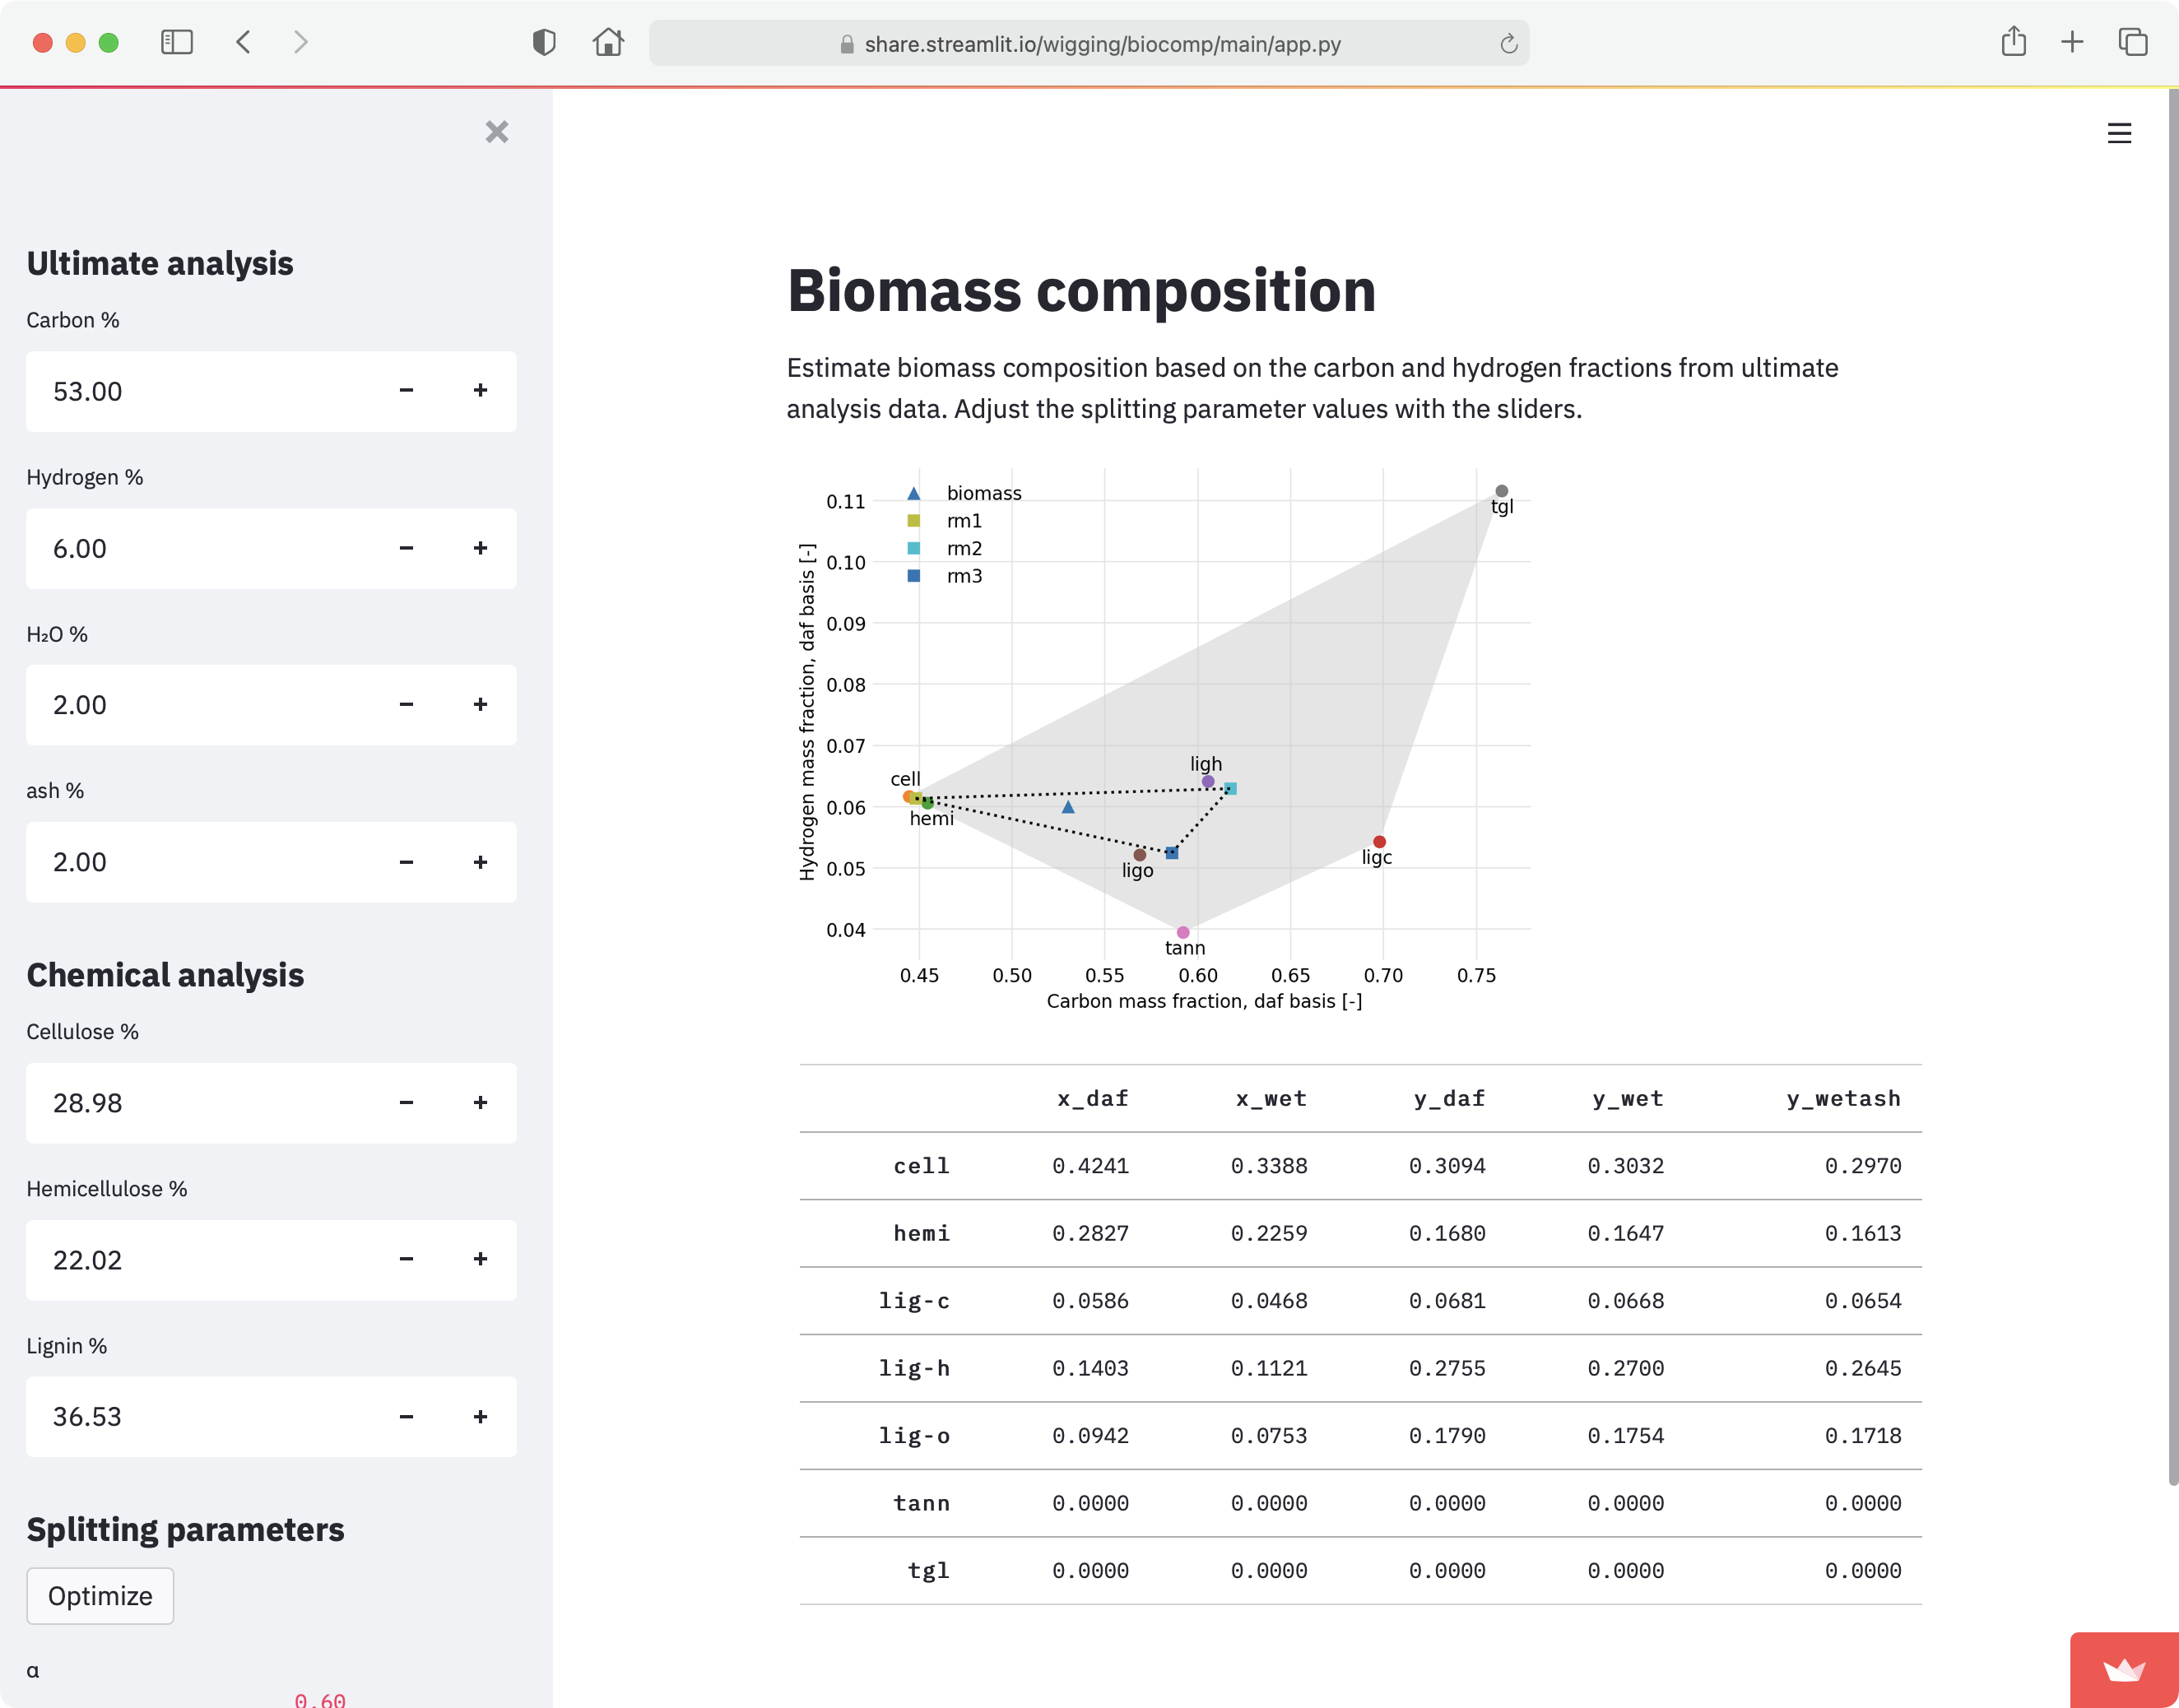
\includegraphics[width=0.9\textwidth]{figures/webtool.png}
    \caption{An online tool to estimate biomass composition from ultimate and chemical analysis data for use with the Debiagi et al. pyroylsis kinetics scheme.}
    \label{fig:webtool}
\end{figure}
